% Copyright (c) 2014,2016,2018 Casper Ti. Vector
% Public domain.

\chapter{引言}
\section{晶体和 X 射线的相互作用}

在 \textcite{rietveld1969}关于全谱拟合的工作之后,晶体结构解析常常被分为
结构测定和结构精修两个主要步骤:前者对空间群、晶胞参数、晶胞化学式和
原子坐标等等基本参数进行大致的确定,而后者不仅对这些参数进行精细的调整,
而且也对由仪器灵敏度、衍射峰形等等更多因素决定的各种参数进行拟合,
以使所有这些参数和实际测得的整个衍射谱之间达到最大程度的吻合。
本文主要讨论通过 X 射线粉末衍射测定晶体结构的问题,
而本节将对晶体和 X 射线之间相互作用的理论进行简要的总结。

一般而言,在对晶体样品进行 X 射线衍射实验时,光源、检测器到样品的距离都远大于
样品的尺寸,而 X 射线的波长和晶胞的尺寸在相近的数量级上,因此样品对 X 射线的
散射满足 Fraunhofer 远场条件\parencite{zhong2003}。晶体和 X 射线之间的相互
作用主要是其中电子云对 X 射线的散射,而在电子云对单波长电磁波的远场散射中,
散射波的复振幅 $A$ 和散射体的电子密度分布 $\rho$ 之间满足以下的 Fourier 关系:
\begin{equation}
	A(\vec{q}) \propto f(\vec{q}) = \int\rho(\vec{r})
		\iee^{2\uppi\eye\vec{q}\cdot\vec{r}}\dif\tau_\vec{r}\mccomma
\end{equation}
其中 $\vec{q}$ 为散射向量,$\tau_\vec{r}$ 为正空间的体积元,$f$ 即%
\myterm{散射因子}。由此结合 Fourier 变换的可加性和位移{--}相移关系,
并忽略 X 射线的次级散射\parencite[4]{pecharsky2009},
可知原点在 $(0, 0, 0)$ 的单个晶胞的散射因子正是其\myterm{结构因子}
\begin{equation}
	F(\vec{q}) = \sum_j f_j(\vec{q})
		\iee^{2\uppi\eye\vec{q}\cdot\vec{r}_j}\mccomma
\end{equation}
其中 $j$ 为单个原子\footnote{%
	在讨论晶体结构时,常常将其中的离子也称为“原子”,而本文中也采用这一约定。%
}的编号,$f_j$ 和 $\vec{r}_j$ 分别为其原子散射因子和坐标。

再次在忽略次级散射后利用 Fourier 变换的可加性和位移{--}相移关系,
可得整块晶体的散射因子为
\begin{equation}
	\sum_j F(\vec{q})\iee^{2\uppi\eye\vec{q}\cdot\vec{r}_j}
	= F(\vec{q})\sum_j\iee^{
		2\uppi\eye(h\vec{a}^* + k\vec{a}^* + l\vec{a}^*)
		\cdot(u_j\vec{a} + v_j\vec{b} + w_j\vec{c})
	} = F(\vec{q})\sum_j\iee^{2\uppi\eye(hu_j + kv_j + lw_j)}
	\mccomma\label{eq:amp-sf}
\end{equation}
其中 $\{\vec{a}, \vec{b}, \vec{c}\}$、$\{\vec{a}^*, \vec{b}^*, \vec{c}^*\}$
分别为正空间和倒空间晶格的基向量组\footnote{%
	本文统一使用不含 $2\uppi$ 因子的倒基向量定义%
	\parencite[1]{prince2004},以下不再特别说明。%
},$j$ 为单个晶胞的编号,$\vec{r}_j$ 为该晶胞的原点坐标。假设有一个
晶胞的原点在 $(0, 0, 0)$,那么为了使来自所有晶胞的散射波发生相长干涉,%
$hu_j + kv_j + lw_j$ 应均为整数;又由晶体\footnote{%
	国际晶体学联合会\parencite{iucr1992}目前将晶体定义为“any solid having
	an essentially discrete diffraction diagram”,即包括具有平移周期性的
	常规晶体和不具有平移周期性的准晶\parencite{shechtman1984};然而,
	本文只讨论常规晶体的结构测定,而本文所称的“晶体”也一律指常规晶体。%
}的平移周期性可知 $u_j$、$v_j$、$w_j$ 均为整数,因此 $h$、$k$、$l$ 也应为整数。

由此可知,产生衍射峰的散射向量必须是倒晶格向量,这正是我们熟知的 Laue 条件;
在满足 Laue 条件时,由 (\ref{eq:amp-sf}) 式进一步可知总散射因子正比于
结构因子。在具体的衍射实验中,还有其它的许多因素影响实际测得的衍射谱%
\parencite{liang2011}:例如衍射装置的几何结构主要由 Lorentz{--}极化因子
反映,粉末衍射中倒易向量模相等的衍射峰互相重叠由多重度因子反映,此外还有
热振动、样品吸收等等多种影响因素。但无论如何,由本节的推导可见,结构因子和
晶胞中原子排布之间的紧密联系决定了对结构因子的处理是晶体结构测定的核心。

\section{倒空间法求解晶体结构}\label{sec:reci-meth}

因为 Fourier 变换具有可逆性,如果获得了各主要衍射峰所对应结构因子的值,
就可以通过逆变换获得晶胞内的电子密度分布,从而得到晶胞内各原子的位置;
然而在进行衍射实验时,对 X 射线的测量会丢失相位信息,因为仪器测量到的只是
衍射峰的强度,而其正比于结构因子振幅的平方。因此如果要得到完整的结构因子,
就须要设法重建结构因子的相位,而重建结构相位的数值依据就是结构振幅。
这正是结构测定中\myterm{倒空间法}的基本思路,其名字源于对倒空间中结构振幅
的提取;以下对目前在用粉末衍射数据进行结构测定\parencite{david2002}%
的算法中被最广泛使用的几种倒空间法进行简要的总结,其中各方法的
常用软件列表可以参考下文中相应的文献。

\myterm{Patterson 法}\parencite{rossmann2001}:
对结构振幅的平方(正比于衍射峰的强度)进行 Fourier 变换,可以得到
Patterson 函数,后者可以理解为电子密度分布的自卷积或“自关联”函数
\begin{equation}
	P(\vec{R}) = \int\,\rho(\vec{r})\rho(\vec{r + R})\dif\tau_\vec{r}\mcstop
\end{equation}
含 $n$ 个原子的晶胞会在 Patterson 函数中产生 $n^2$ 个峰,
因此即使不考虑峰的重叠问题,一般而言总的 Patterson 峰数仍然会很大。
除了原点处的强峰之外,具有高强度的 Patterson 峰主要由含重原子的原子对产生,
所以由这些重原子峰可以确定重原子的位置,而由重原子的位置结合
Patterson 函数中更多的信息便可以进一步推测整个晶胞中各原子的位置。

\myterm{直接法}\parencite{giacovazzo2001}:
根据电子密度分布函数的正定性和原子性,可以得到不同衍射峰所对应
(为抵消高角度峰的强度衰减)归一化结构因子 $E_\vec{q}$ 以及单位结构因子
$U_\vec{q}$ 之间的一系列数值关系,其中最重要的是一组根据给定衍射峰的
结构振幅对一些相关衍射峰结构相位的取值进行限制的不等式关系,
以及一组概率性的等式关系:例如对 $P\bar1$ 空间群有
\vspace{\slop{-0.05em}}
\begin{equation}
	U_\vec{q} ^ 2 \leq (1 + U_{2\vec{q}}) / 2\mccomma
	\vspace{\slop{-0.05em}}
\end{equation}
而以下的正切公式(其中 $G_\vec{k} \propto
|E_\vec{q}||E_\vec{k}||E_{\vec{q}-\vec{k}}|$)给出最概然的结构相位
\vspace{\slop{0.09em}}
\begin{equation}
	\tan\arg{E_\vec{q}} = \frac%
	{\sum_\vec{k} G_\vec{k} \sin(\arg{E_\vec{k}} + \arg{E_{\vec{q}-\vec{k}}})}%
	{\sum_\vec{k} G_\vec{k} \cos(\arg{E_\vec{k}} + \arg{E_{\vec{q}-\vec{k}}})}
	\mcstop
	\vspace{\slop{0.09em}}
\end{equation}
在实际求解时,在计算 $E_\vec{q}$、$U_\vec{q}$ 后,选出较强衍射峰所组成的
$\{\vec{q}, \vec{k}, \vec{q}-\vec{k}\}$ 三元组,根据上述的不等式和等式关系
可以对其中一小部分结构相位的符号甚至具体数值进行直接估计;在此之后,通过
迭代性地应用等式关系和不等式关系,就可以对各主要衍射峰的结构相位进行重建。

\myterm{电荷反转法}\parencite{palatinus2013}:
在满足 Friedel 定律\parencite[218-220]{pecharsky2009}的前提下,
如果对各结构因子赋予随机相位,由此得到的电子密度分布往往不具备正定性
和原子性。为了满足正定性条件,可以强行将负电子密度部分的符号反转;
此外为了引入随机微扰,考虑到实际电子密度分布的集中性(可以认为是
由原子性导致的),实际计算时会将电子密度小于某一预设正值的部分进行
反转。在这样修改电子密度分布之后,用原结构振幅结合反演得到的结构相位,
得到的结构因子又可以通过同样的流程产生新的结构相位,如此便可进行迭代;
根据实际测试,对于许多衍射谱,通过上述迭代算法可以获得满意的结构相位。

一般而言,为了能使用倒空间法正确求解晶体结构,衍射谱中可确定结构振幅的
衍射峰数须要远多于晶胞中待定的原子数,因此衍射数据通常需要较高的分辨率,
这在上述几种算法的参考文献中多少有所提及。在对粉末衍射数据使用倒空间法时,
还须要设法分离互相重叠的衍射峰,这又使得粉末数据需要比单晶数据更高的分辨率。
在很多情况下,高分辨的衍射数据很难获得,特别是对纳米材料,即使应用
同步辐射也很难获得高质量的单晶衍射数据;在没有高分辨衍射数据的情况下,
常常不得不使用正空间法求解晶体结构,而正空间法就是本文将要讨论的主题。

\section{正空间法和等效点系组合法}\label{sec:dspace-epc}

求解晶体结构的另一种主要思路是直接从原子坐标建立试探性的晶体模型,然后计算
晶体模型所对应的衍射谱,将计算得到的衍射谱和实际测得的衍射谱比对,并根据结果
设法对晶体模型进行优化,直到获得满意的模型。这正是\myterm{正空间法}%
\parencite{cerny2007}的思路,后者是除了上文中讨论的倒空间法之外,
用粉末衍射数据进行结构测定的主要算法;显然,正空间法并不依赖对结构相位的估计,
而且甚至不需要单个衍射峰的结构振幅,因此其特别适合处理低分辨的衍射数据,
以及衍射峰重叠严重的粉末数据。

在计算机尚未被广泛应用于科学计算的年代,晶体结构测定仍严重依赖手动计算和尝试,
而对于晶体模型的优化也极大程度地依赖具有极强技巧性(乃至艺术性)的人工处理:
例如在包括\textcite{lu1965},\textcite{reddy1965}在内的许多先驱的工作中,
晶体学家在大致确定各原子的等效点系组合(参考下文和第 \ref{ssec:epc-discus}
小节)之后,通过立体几何的原理确定具体的原子坐标。在现代的正空间法中,
尝试性晶体模型的建立和优化仍然不可或缺,只是往往被自动化的计算机程序
以极高的频率反复进行;因为这样的原因,正空间法也往往被称为尝试法%
\parencite{wolfson1997}和模型法\parencite{cerny2007}。

从数学上容易看出,正空间法将结构测定抽象为寻找使一%
\myterm{目标函数}最小化的原子坐标组合
\begin{equation}
	\mat{x} = (x_1, y_1, z_1, x_2, y_2, z_2, \cdots, x_n, y_n, z_n)^\tee
\end{equation}
的全局最优化问题,其中 $n$ 是晶胞内的原子数,而目标函数中最重要的部分是
表征计算谱和实际谱之间差异的 \myterm{Bragg $R$ 因子}。为了利用计算机
自动化地寻找合理的 $\mat{x}$,现代的正空间法使用各种最优化算法,
例如模拟退火\parencite{david2006}、并行回火\parencite{cerny2007}、
遗传算法\parencite{shankland1997}等等来求解上述的问题,
因此正空间法的另一个别称是全局最优化法\parencite[252]{david2002}。

若直接以晶胞中所有 $n$ 个原子的坐标组合为正空间法中全局最优化的自变量,
则最优化问题的维数为 $3n$;注意到最优化问题中搜索空间的规模随其维数指数增长,
设法尽量降低维数显然很有必要。对于成键关系大部分已知的结构,例如分子晶体%
\parencite{andreev1997}、框架晶体\parencite{falcioni1999}以及部分其它类型的
晶体\parencite{favre2002},可以将原子团的平移、振动、转动等等自由度作为自变量,
利用原子团的相对刚性来降低最优化问题的维数,并对键长、键角进行适当限制以进一步
缩小搜索空间。相比之下,在求解成键关系总体未知的结构时,关于成键关系的
先验知识就缩小搜索空间而言作用很有限;对于这类结构,等效点系组合法%
\parencite{deng2009}常常是一种有效的手段,而下文就将对其进行简要的总结。

在空间群和晶胞化学式已知\footnote{%
	本文主要考虑对已指标化粉末衍射数据的处理,因此在讨论结构测定时一般假定
	晶胞参数和空间群是已知的,或至少能确定空间群在某个比较小的范围之中。此外,
	因为结构测定所用样品的名义组成一般是已知的,在确定晶胞参数之后常常可以
	通过密度测量获得晶胞的化学组成,所以本文一般也假定晶胞化学式是已知的。%
}的前提下,考虑到绝大多数晶体中晶胞的对称性,可以将晶胞中独立原子的坐标
作为自变量,从而极大地降低最优化问题的维数。为了得到独立原子的具体列表,
我们须要将晶胞中的原子分配到可用的 Wyckoff 位置上,而每一种分配方案就是一种%
\myterm{等效点系组合}(equivalent position combination,简称 EPC)。例如对于
\ce{PbSO4}($Pnma$,$Z = 4$),因为 $Pnma$ 空间群有 $4a$、$4b$、$4c$、$8d$
等共 4 种 Wyckoff 位置,为了满足正确的晶胞化学式,其中原子有且仅有 35 种 EPC:
\vspace{\slop{0.15em}}
\begin{itemize}
	\item \ce{Pb^{2+}}: $4a\times1$; \ce{S^{6+}}: $4b\times1$;
		\ce{O^{2-}}: $4c\times4$(8 维);
	\item \ce{Pb^{2+}}: $4a\times1$; \ce{S^{6+}}: $4b\times1$;
		\ce{O^{2-}}: $4c\times2 + 8d\times1$(7 维);
	\item ……
	\item \ce{Pb^{2+}}: $4c\times1$; \ce{S^{6+}}: $4c\times1$;
		\ce{O^{2-}}: $4c\times2 + 8d\times1$(11 维,正确 EPC)。
	\item \ce{Pb^{2+}}: $4c\times1$; \ce{S^{6+}}: $4c\times1$;
		\ce{O^{2-}}: $8d\times2$(10 维)。
\end{itemize}
\vspace{\slop{0.15em}}
原先 72 维的最优化问题被转化为 35 个介于 6--12 维之间的最优化问题,
可见 EPC 法极大地缩减了 \ce{PbSO4} 结构求解问题的总规模。

正空间法和 EPC 法的常用软件列表参考第 \ref{sec:atom-bump} 小节;此外有必要指出,
随着近年来双空间迭代技术,如电荷反转法(参考第 \ref{sec:reci-meth} 节),%
\textcite{altomare2008b}的直接法{--}模拟退火混合方案和 \textcite{ma2004}的
UACIEM 方法等等的发展,倒空间法和正空间法之间的界限正在逐步地模糊。然而,
双空间迭代法目前的发展趋势并非是取代倒空间法或正空间法,而是让这两类算法
更加紧密地互相结合,因此针对后两类算法本身的研究仍然是具有重要意义的。

\section{原子重叠问题和 \emph{decryst}}\label{sec:atom-bump}

正空间法遇到的一个重要问题是随机产生的晶体模型在化学上不合理,而其中最常见的情况
之一是\myterm{原子重叠}(atom bumping),即产生的模型中一些原子对的间距明显小于
化学上允许的下限,而且这些模型中一部分甚至具有和正确模型相近的 Bragg $R$ 因子。
例如对于 \ce{PbSO4} 的正确等效点系组合(EPC),如果试图通过最小化 $R$ 因子来
求解原子坐标,最终得到的结果往往类似于图 \ref{fig:pso-bump}:虽然正确的
晶体模型中没有原子重叠,但是绝大部分解模型中有严重的原子重叠。对于成键关系
大部分已知的结构,通过对键长、键角等等参数的限制,可以极大地减轻这一问题;
然而对于成键关系总体未知的结构,这一方法的效果很有限。因此为了尽量自动化地
处理原子重叠,我们迫切需要一种具有通用性的机制在全局最优化的过程中高效地
实时检测和排除存在原子重叠的模型,而本文第 \ref{chap:cryst-cd} 章将要
讨论的就是本人\parencite{liu2017}提出的自动化排除原子重叠的机制。

\begin{figure}[htbp!]\bfcmd
\ffigbox{\begin{subfloatrow}[3]
	\ffigbox[\FBwidth]{%
		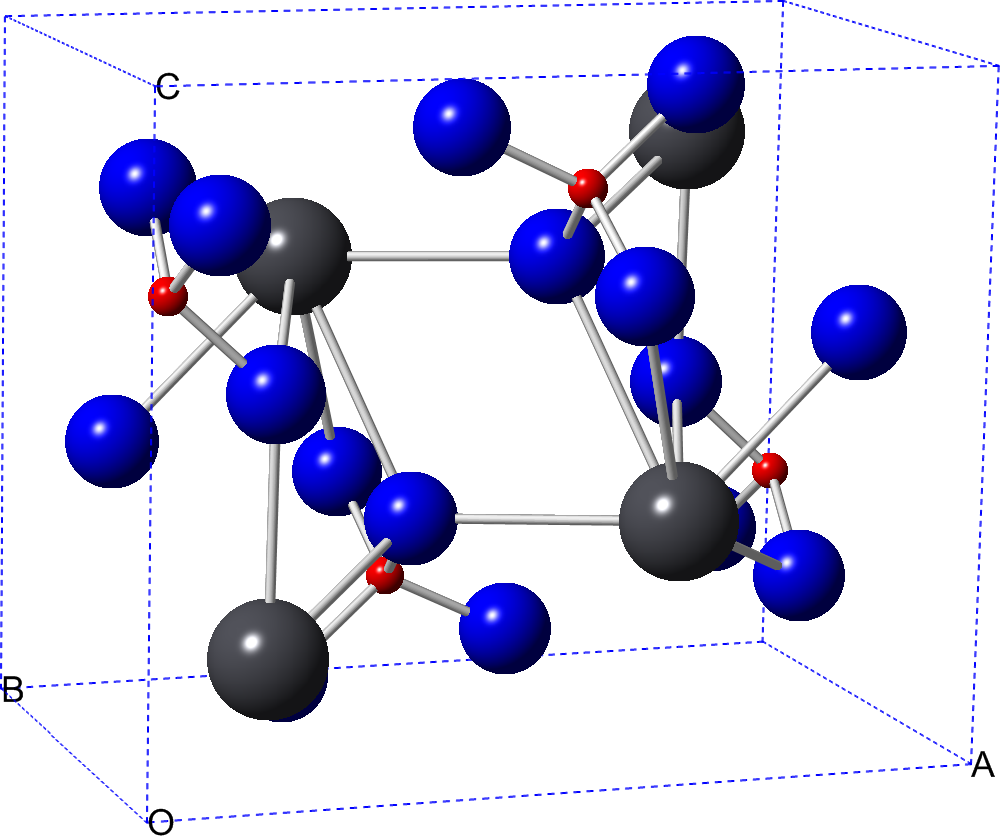
\includegraphics[width = 0.3\textwidth]{img/pso-bump-1}%
	}{\caption{$R = 0.1285$}}
	\ffigbox[\FBwidth]{%
		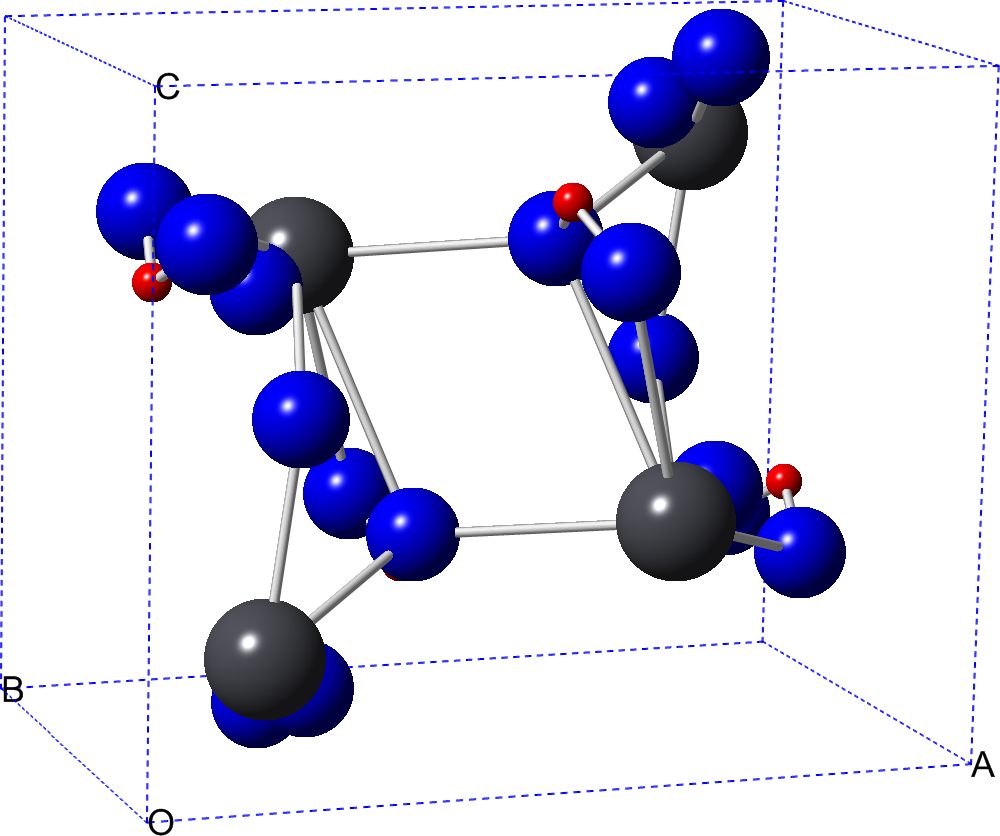
\includegraphics[width = 0.3\textwidth]{img/pso-bump-2}%
	}{\caption{$R = 0.0971$}}
	\ffigbox[\FBwidth]{%
		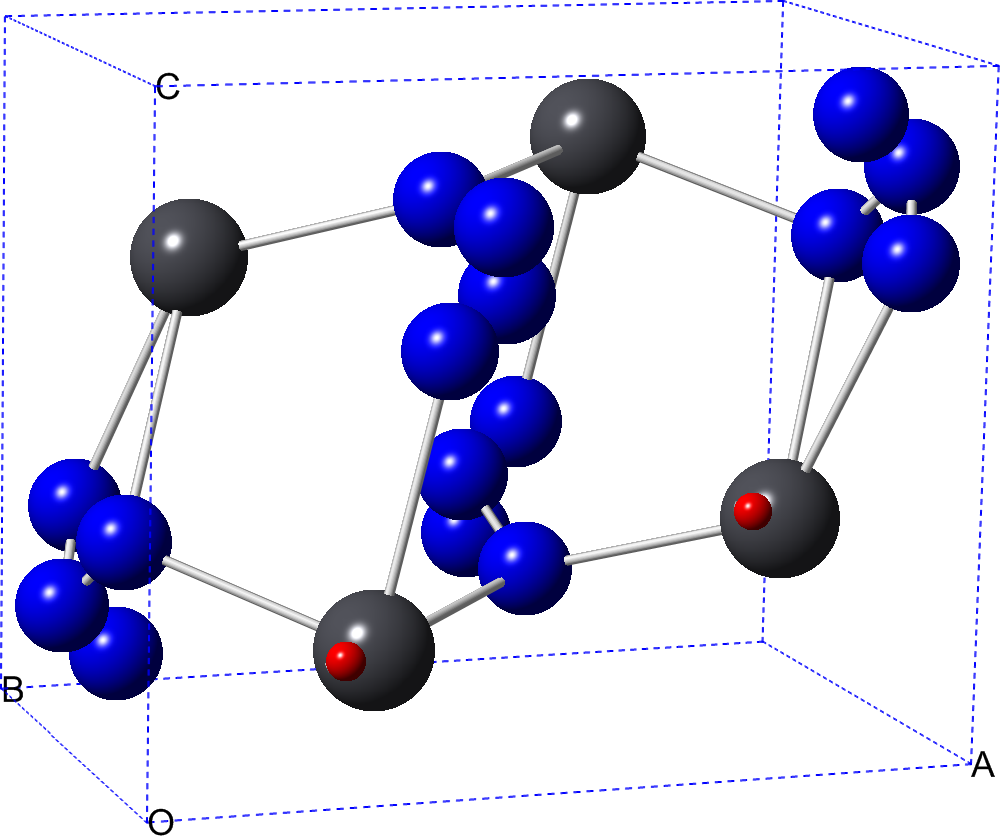
\includegraphics[width = 0.3\textwidth]{img/pso-bump-3}%
	}{\caption{$R = 0.1140$}}
\end{subfloatrow}}{\caption[\ce{PbSO4} 的几种晶体模型]{%
	\ce{PbSO4} 的几种晶体模型,其中只有 (a) 正确
	(数据来源参考第 \ref{ssec:cd-eval} 小节)%
}\label{fig:pso-bump}}
\end{figure}

现有的使用正空间法从粉末衍射数据求解晶体结构的主流软件,如 \emph{FOX}%
\parencite{favre2002}、\emph{DASH}\parencite{david2006}、\emph{EXPO}%
\parencite{altomare2013}等等多数适合求解成键关系大部分已知的结构,但在求解
成键关系总体未知的结构时不甚有效;针对后一类结构的求解,\textcite{deng2011}%
基于 EPC 法开发了 \emph{EPCryst} 这一软件,但其对原子重叠的处理方式是在
全局最优化步骤完成之后对解模型进行筛选,因此排除原子重叠的效率相当低。
考虑到以上的现状,本人开发了 \emph{decryst}\parencite{liu2018},
以使上述的排除原子重叠的机制在求解未知结构的过程中发挥实际的作用。

受 Unix 中 \verb|make| 程序\parencite{feldman1979}的启发,本人在
\emph{decryst} 中将增量计算的技术应用于最优化步骤中,使其性能得到了很大的提升;
除此之外,考虑到目前科学计算(乃至通用计算)中大规模并行化的发展趋势,
本人在设计 \emph{decryst} 时也加入了对并行和分布式计算的支持,
使之可以通过同时利用多个处理器实现对晶体结构测定的进一步加速。
因为各 EPC 在计算上互相独立,而多数未知结构的 EPC 数很大,
可以认为 EPC 法对搜索空间的缩减作用和 EPC 任务的大规模并行化将为
求解成键关系总体未知的结构带来前所未有的机遇。针对这些内容,本文第
\ref{chap:decr-theory} 章将展开讨论 \emph{decryst} 的基本设计和实现。

第 \ref{sec:dspace-epc} 节提到,在早期的利用正空间法进行结构测定的工作中,
晶体学家通过具有很强经验性和技巧性的手段对备选的 EPC 进行分析,从而筛除掉其中
不可能产生合理晶体模型的 EPC。在 \emph{EPCryst} 中,用户可以通过对随机晶体模型
Bragg $R$ 因子的统计分析实现对 EPC 的简单筛选;在此基础之上,\emph{decryst}
在筛选 EPC 时使用包含原子重叠的目标函数,因此可以在筛选中同时考虑 $R$ 因子和
原子重叠两种因素。\emph{decryst} 的设计追求简洁、灵活,其在现有自动化工具
的配合之下可以实现相当复杂的求解流程,如重原子法和多步骤的精细 EPC 筛选。
针对以上问题,本文第 \ref{chap:decr-usage} 章将比较详细地讨论 \emph{decryst}
的使用方法和常用技巧。

最后有必要指出,除了 EPC 法之外,\emph{FOX} 中的动态占据率校正(dynamical
occupancy correction)也是一种处理特殊位置上原子的有效方法,但其更适用于
以原子团为基础的晶体模型。对于成键关系总体未知的结构,该方法就降低最优化
问题的复杂度而言效果有限,因此在实用性上不如 EPC 法。

\begin{rquote}{0.2\textwidth}
	Zum Nutzen und Gebrauch der Lehrbegierigen
	Musicalischen Jugend, als auch derer in diesem
	studio schon habil seyenden besonderem Zeitvertreib [...]
\end{rquote}
\rightline{--- J.\ S.\ Bach, ``\emph{Das Wohltemperierte Klavier}''}

% vim:ts=4:sw=4
